\begin{enumerate}
    \item If $\sin \theta=0$, then the value of $\tan^2\theta+\cot^2\theta$ is
    \begin{enumerate}
        \item $2$
        \item $4$
        \item $1$
        \item $\frac{10}{9}$
    \end{enumerate}
    \item The value(s) of $k$ for which the quadratic equation 
    \begin{align}
        3x^2 - kx + 3 = 0
    \end{align}
    has equal roots, is (are) 
    \begin{enumerate}
        \item $6$
        \item $-6$
        \item $\pm6$
        \item $9$
    \end{enumerate}
    \item $5\tan^2 \theta - 5\sec^2\theta = \underline{\hspace{2cm}}$
    \item If $\alpha$, $\beta$ are zeroes of the polynomial $2x^2 - 5x - 4$, then $\frac{1}{\alpha}+\frac{1}{\beta}$.
    \item In  \figref{fig:as.jpeg}, a tower stands vertically on the ground. From a point on the ground, which is $80m$ away from the foot of the tower, the angle of elevation of the tower is found to be $30\degree$. Find the height of the tower.
    \begin{figure}[H]
        \centering
        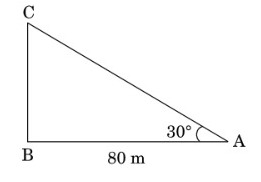
\includegraphics[width=70mm]{figs/as.jpeg}
        \caption{as.jpeg}
        \label{fig:as.jpeg}
    \end{figure}
    \item Solve
    \begin{align}
        9x^2 - 6a^2x + a^4 - b^4 = 0
    \end{align}
    using the quadratic formula.
    \item Show that 
    \begin{align}
        \cos(38\degree) \cos(52\degree) - \sin(38\degree)\sin(52\degree) = \cos(90\degree).
    \end{align}
    \item Prove that 
    \begin{align}
        \frac{\sin\theta}{\cot\theta+\csc\theta} = 2+\frac{\sin\theta}{\cot\theta-\csc\theta}.
    \end{align}
    \item Given 
    \begin{align}
        15 \cot (A) = 8,
    \end{align}
    find the values of $\sin (A)$ and $\sec (A)$.
    \item The angles of depression of the top and bottom of a tower as seen from the top of a $60\sqrt{3}m$ high cliff are $45\degree$ and $60\degree$ respectively. Find the height of the tower. (Use $\sqrt{3}=1.73$)
    \item $A$ and $B$ jointly finish a piece of work in $15$ days. When they work separately, $A$ takes $16$ days less than the number of days taken by $B$ to finish the same piece of work. Find the number of days taken by $B$ to finish the work.
    \item If the polynomial
    \begin{align} 
        f(x) = 3x^4 - 9x^3 + x^2 + 15x + k
    \end{align}
    is completely divisible by $3x^2 - 5$, then find the value of $k$. Using the quotient obtained, find two zeroes of the polynomial.
    \item Find all the zeroes of the polynomial
    \begin{align}
        f(x)x^4 - 8x^3 + 23x^2 - 28x + 12
    \end{align}
    if two of its zeroes are $2$ and $3$.  
    \item Find the value of $m$ for which the quadratic equation
    \begin{align}
        (m-1)x^2 + 2(m-1)x + 1 = 0
    \end{align}
    has two real and equal roots. 
    \item Solve the following quadratic equation for $x$ 
    \begin{align}
        \sqrt{3}x^2 + 10x + 7\sqrt{3} = 0
    \end{align}
    \item  The product of Rehan's age (in years) $5$ years ago and his age $7$ years from now is one more than twice his age. Find his present age.
    \item The angle of elevation of the top of a building from the foot of the tower is $30\degree$ and the angle of elevation of the top of the tower from the foot of the building is $60\degree$. If the tower is $50$ meters high, then find the height of the building.
    \item From a point on a bridge across a river, the angles of depression of the banks on opposite sides of the river are $30\degree$ and $60\degree$ respectively. If the bridge is at a height of $3$ meters from the banks, then find the width of the river. 
    \item In \figref{fig:ak}, Gadisar Lake is located in the Jaisalmer district of Rajasthan. It was built by the King of Jaisalmer and rebuilt by Gadsi Singh in the $14$th century. The lake has many Chhatris. One of them is shown below:
    \begin{figure}[H]
        \centering
    	 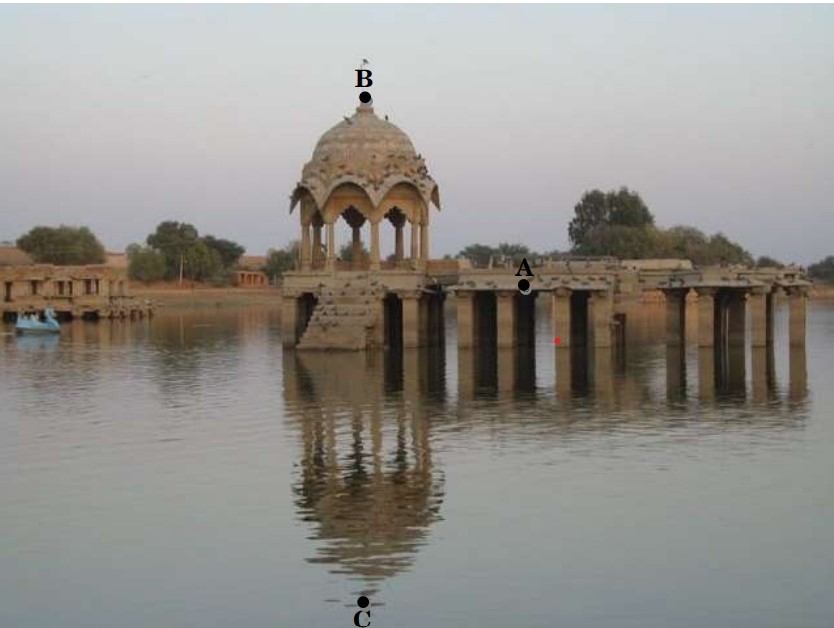
\includegraphics[width=70mm]{figs/ak.jpeg}
        \caption{ak.jpg}
        \label{fig:ak}
    \end{figure}
    Observe the picture. From a point $A$ $h$ meters above the water level, the angle of elevation of the top of Chhatri (point $B$) is $45\degree$ and the angle of depression of its reflection in the water (point $C$) is $60\degree$ . If the height of Chhatri above water level is (approximately) $10$ meters, then 
    \begin{enumerate}
        \item Draw a well-labeled figure based on the above information.
        \item Find the height ($h$) of the point $A$ above water level. (Use $\sqrt{3}=1.73$) 
    \end{enumerate}

    \item Solve the quadratic equation 
    \begin{align}
        x^2 + \sqrt{2}x - 6 = 0
    \end{align}
    for $x$.
    
    \item In \figref{fig:su.jpeg}, from a point on a bridge across a river, the angles of depression of the banks on opposite sides of the river are $30\degree$ and $45\degree$. If the bridge is at a height of $8$ meters from the banks, then find the width of the river.
    \begin{figure}[H]
        \centering
        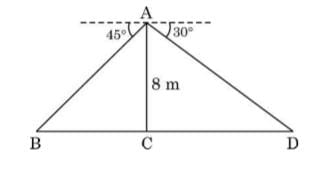
\includegraphics[width=70mm]{figs/su.jpeg}
        \caption{su.jpg}
        \label{fig:su.jpeg}
    \end{figure}
    
    \item A $2$-digit number is such that the product of its digits is $24$. If $18$ is subtracted from the number, the digits interchange their places. Find the numbers.
    
    \item The difference of the squares of two numbers is $180$. The square of the smaller number is $8$ times the greater number. Find the two numbers.
    
    \item Case Study-1:
    
    In \figref{fig:kite.jpeg}, Kite Festival is celebrated in many countries at different times of the year. In India, every year on $14^{th}$ January is celebrated as International Kite Day. On this day, many people visit India and participate in the festival by flying various kinds of kites.
    
    \begin{figure}[H]
	\centering
        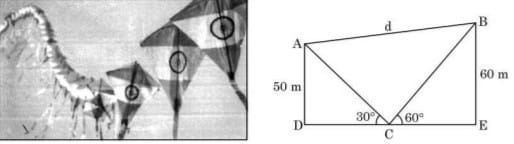
\includegraphics[width=70mm]{figs/kite.jpeg}
        \caption{kites}
        \label{fig:kite.jpeg}
    \end{figure}
    
    In Fig. 5, the angles of elevation of two kites (Point $A$ and $B$) from the hands of a man (Point $C$) are found to be $30\degree$ and $60\degree$ respectively. Taking $AD = 50$ meters and $BE = 60$ meters, find:
    \begin{enumerate}
        \item The lengths of strings used (take them straight) for kites $A$ and $B$ as shown in the figure.
        \item The distance $d$ between these two kites.
    \end{enumerate}
    
    \item Solve the quadratic equation for $x$:
    \begin{align}
        x^2 - 2ax - (4b^2 - a^2) = 0
    \end{align}
    
    \item If the quadratic equation
    \begin{align}
        (1+a^2)x^2 + 2abx + (b^2-c^2) = 0
    \end{align}
    has equal and real roots, then prove that:
    \begin{align}
        b^2 = c^2(1+a^2)
    \end{align}
    
    \item Two boats are sailing in the sea $80$ meters apart from each other towards a cliff $AB$. The angles of depression of the boats from the top of the cliff are $30\degree$ and $45\degree$ respectively, as shown in \figref{fig:boat.jpeg}
    
    \begin{figure}[H]
        \centering
        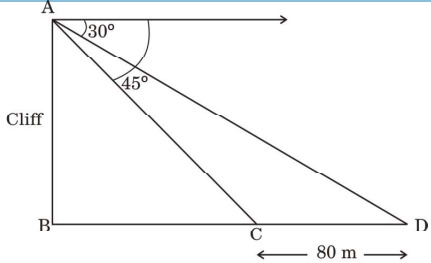
\includegraphics[width=70mm]{figs/boat.edit.jpeg}
        \caption{boat}
        \label{fig:boat.jpeg}
    \end{figure}
    
    Find the height of the cliff.
    
    \item The angle of elevation of the top $Q$ of a vertical tower $PQ$ from a point $X$ on the ground is $60\degree$. From a point $Y$, $40$ meters vertically above $X$, the angle of elevation of the top $Q$ of tower $PQ$ is $45\degree$. Find the height of the tower $PQ$ and the distance $PX$. (Use $\sqrt{3} = 1.73$)
    
    \item Find the value of $k$ for which the quadratic equation
    \begin{align}
        2kx^2 - 40 + 25 = 0
    \end{align}
    has real and equal roots. 
    
    \item Solve for $x$:
    \begin{align}
        \frac{5}{2}x^2 + \frac{2}{5} = 1 - 2x
    \end{align}
    
    \item An Aeroplane at an altitude of $200$ meters observes the angles of depression of opposite points on the two banks of a river to be $45\degree$ and $60\degree$. Find the width of the river. (Use $\sqrt{3} = 1.732$)
    
    \item Find the value(s) of $'p'$ for which the quadratic equation $(px-4)(x-2)$ has real and equal roots.
    
    \item Had Aarush scored $8$ more marks in a Mathematics test, out of $35$ marks, $7$ times these marks would have been $4$ less than the square of his actual marks. How many marks did he get in the test?
    
    \item From the top of an $8$ meter high building, the angle of elevation of the top of a cable tower is $60\degree$ and the angle of depression of its foot is $45\degree$. Determine the height of the tower. (Take $\sqrt{3} = 1.732$).
    
    \item Find the roots of the quadratic equation 
    \begin{align}
        9x^2 - 6\sqrt{2}x + 2 = 0
    \end{align}
    
    \item The product of two consecutive odd positive integers is $255$. Find the integers, by formulating a quadratic equation.
    
    \item Find the value(s) of $k$ for the quadratic equation,
    \begin{align}
        (k+3)x^2 + kx + 1 = 0
    \end{align}
    to have two real and equal roots.
    
    \item As observed from the top of a lighthouse $60$ meters high from the sea level, the angles of depression of two ships are $45\degree$ and $60\degree$. If one ship is exactly behind the other on the same side of the lighthouse, then find the distance between the two ships. (Use $\sqrt{3} = 1.732$)
    
    \item At a point on the level ground, the angle of elevation of the top of a vertical tower is found to be $\alpha$, such that $\tan\alpha = \frac{5}{12}$. On walking $192$ meters towards the tower, the angle of elevation $\beta$ is such that $\tan\beta = \frac{3}{4}$. Find the height of the tower.
    
    \item $\tan^{-1}\frac{1}{\sqrt{3}} - \cot^{-1}\frac{-1}{\sqrt{3}}$
    
    \item Show that the relation $R$ in the set of all real numbers, defined as $R = \{(a,b) : a \leq b^2\}$.
    
    \item Two angles of a triangle are $\cot^{-1}2$ and $\cot^{-1}3$. The third angle of the triangle is?
    
    \item Solve for $x$:
    \begin{align}
        \sin^{-1}(1-x) - 2 \sin^{-1} x = \frac{\pi}{2}
    \end{align}
    \item Find the present value of a perpetuity of \rupee~18,000 at the end of $6$ months if it is worth $8\%$ p.a. compounded semi-annually.
    
    [Given that: $1.00833^{12} = 1.1047$]
    
    \item Find the effective rate which is equivalent to a nominal rate of $10\%$ p.a. compounded monthly.
    
    [Given that: $1.00833^{12} = 1.1047$]
    
    \item Abhay bought a mobile phone for \rupee~30,000. The mobile phone is estimated to have a scrap value of \rupee~3,000 after a span of $3$ years. Using the linear depreciation method, find the book value of the mobile phone at the end of $2$ years.
    
    \item Madhu exchanged her old car valued at \rupee~1,50,000 with a new one priced at \rupee~65,000. She paid \rupee~x as a down payment, and the balance in $20$ monthly equal installments of \rupee~21,000. The rate of interest offered to her is $9\%$ p.a. Find the value of $x$.
    
    [Given that: $1.0075^{-20} = 0.86118985$]
    
    \item Calculate the EMI under the 'Flat Rate System' for a loan of $\rupee~5,00,000$ with $10\%$ annual interest rate for $5$ years.
    
    \item A machine costing \rupee~2,00,000 has an effective life of $7$ years, and its scrap value is \rupee~30,000. What amount should the company put into a sinking fund earning $5\%$ p.a., so that it can replace the machine after its usual life? Assume that a new machine will cost \rupee~3,00,000 after $7$ years.
    
    [Given that: $(1.05)^7 = 1.407$]
    
    \item A start-up company invested \rupee~3,00,000 in shares for $5$ years. The value of this investment was \rupee~3,50,000 at the end of the second year, \rupee~3,80,000 at the end of the third year, and on maturity, the final value stood at \rupee~4,50,000.Calculate the Compound Annual Growth Rate (CAGR) on the investment.
    
    [Given that: $(1.5)^\frac{1}{5} = 1.084$]
\end{enumerate}
